This section will describe the actors and some actions the actor perform, in order to understand what they do in application domain, from this some basic requirements of the systems functionalities and interfaces can formulated. The requirements ensure that the system is usable in the application domain.

\subsection{Actors}
There are two actors of this system; an administrator which could be a
bartender or a bar owner in charge of the music, and a guest wanting
to request and affect the music being played at the venue. Further information about these actors are presented in the below tables for respectively administrators and guests. Based on these actors, actor tables and usage diagrams has been made, see \cref{tab:actorTable,fig:UsageAdmin,fig:UsageUser}. These describe the possible actions each actor can take in the system.

\begin{table}[hbtp]
\centering
\begin{tabular}{lcc}
\toprule
\textbf{Use case}  & Administrator                      & Guest
\\
\midrule
play music         & \checkmark                         &                      \\
stop music         & \checkmark                         &                      \\
next track         & \checkmark                         &                      \\
add restriction    & \checkmark                         &                      \\
remove restriction & \checkmark                         &                      \\
check out          &                                    & \checkmark           \\
check in at venue  &                                    & \checkmark           \\
vote               &                                    & \checkmark           \\
cancel vote        &                                    & \checkmark           \\
influence volume   & \checkmark                         & \checkmark
\\
\bottomrule
\end{tabular}
\caption{Actor table for the project.}\label{tab:actorTable}
\end{table}

\actortable{Administrator}{
    \textbf{Purpose:} A person that protects the interests of the venue and is responsible for the music. He or she wants to be able to have control over the system, what kind and in which order music is being enqueued and what is currently playing.

    \textbf{Characteristics:} Has a preference or a theme of music that the individual is following, set by the organisation or the individual itself. Works at the venue and has a reasonable high technical level or the ability and motivation to be taught the use of the system.

    \textbf{Possible usages:} Administrator 1 is very open minded for all requests and votes from users and only sets the bare minimum restrictions to maintain the theme of the venue.

		Administrator 2 completely controls the playlist by adding, removing and rearranging tracks to completely fit the venue's preferences and what is played. He is very restrictive and only accepts requests and votes that he agrees with.\\\\
		For a diagram of possible usages, see \cref{fig:UsageAdmin}.
}

\begin{figure}[hbtp]
  \centering
  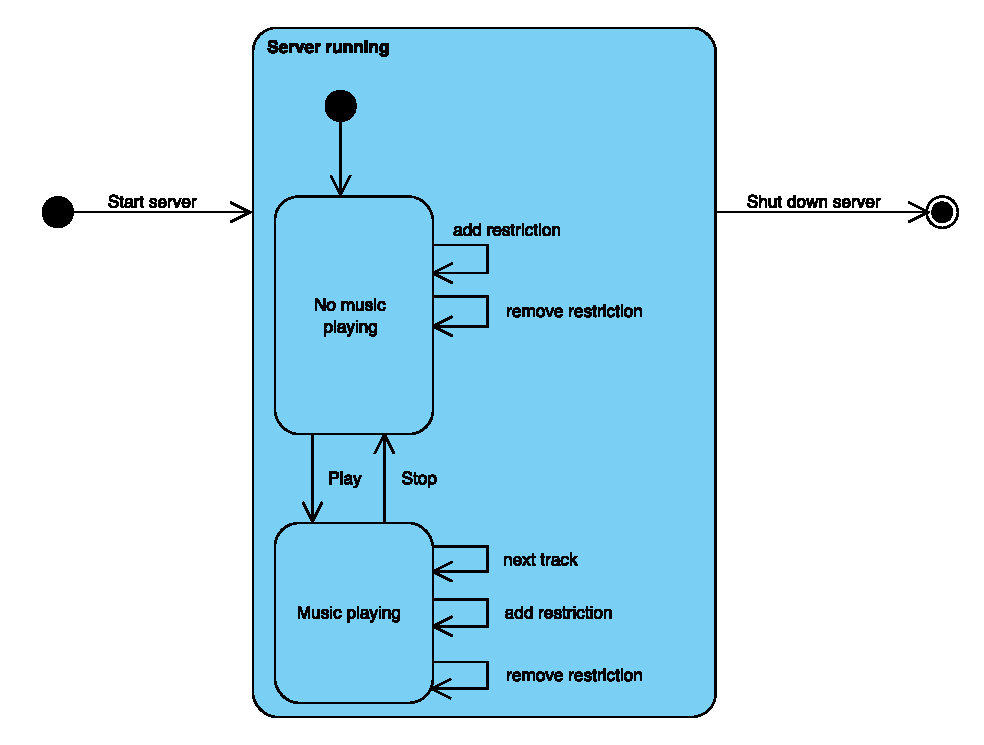
\includegraphics[width=1.1\textwidth]{Images/UsageAdmin.pdf}
  \caption{Usages for a administrator.}\label{fig:UsageAdmin}
\end{figure}

\actortable{Guest}{
    \textbf{Purpose:} Wants to influence the playlist and listen to preferred tracks at a venue.

    \textbf{Characteristics:} Has a music preference possibly different from the administrator and/or the specific theme at the specific venue. Varying technical level but with the ability to use his or her smartphone.

    \textbf{Possible usages:} Guest 1 only requests tracks to the playlist but rarely votes on other users tracks.

		Guest 2 only votes on tracks and does not use the feature of requesting tracks.\\\\
		For a diagram of possible usages, see \cref{fig:UsageUser}.
}

\begin{figure}[hbtp]
  \centering
  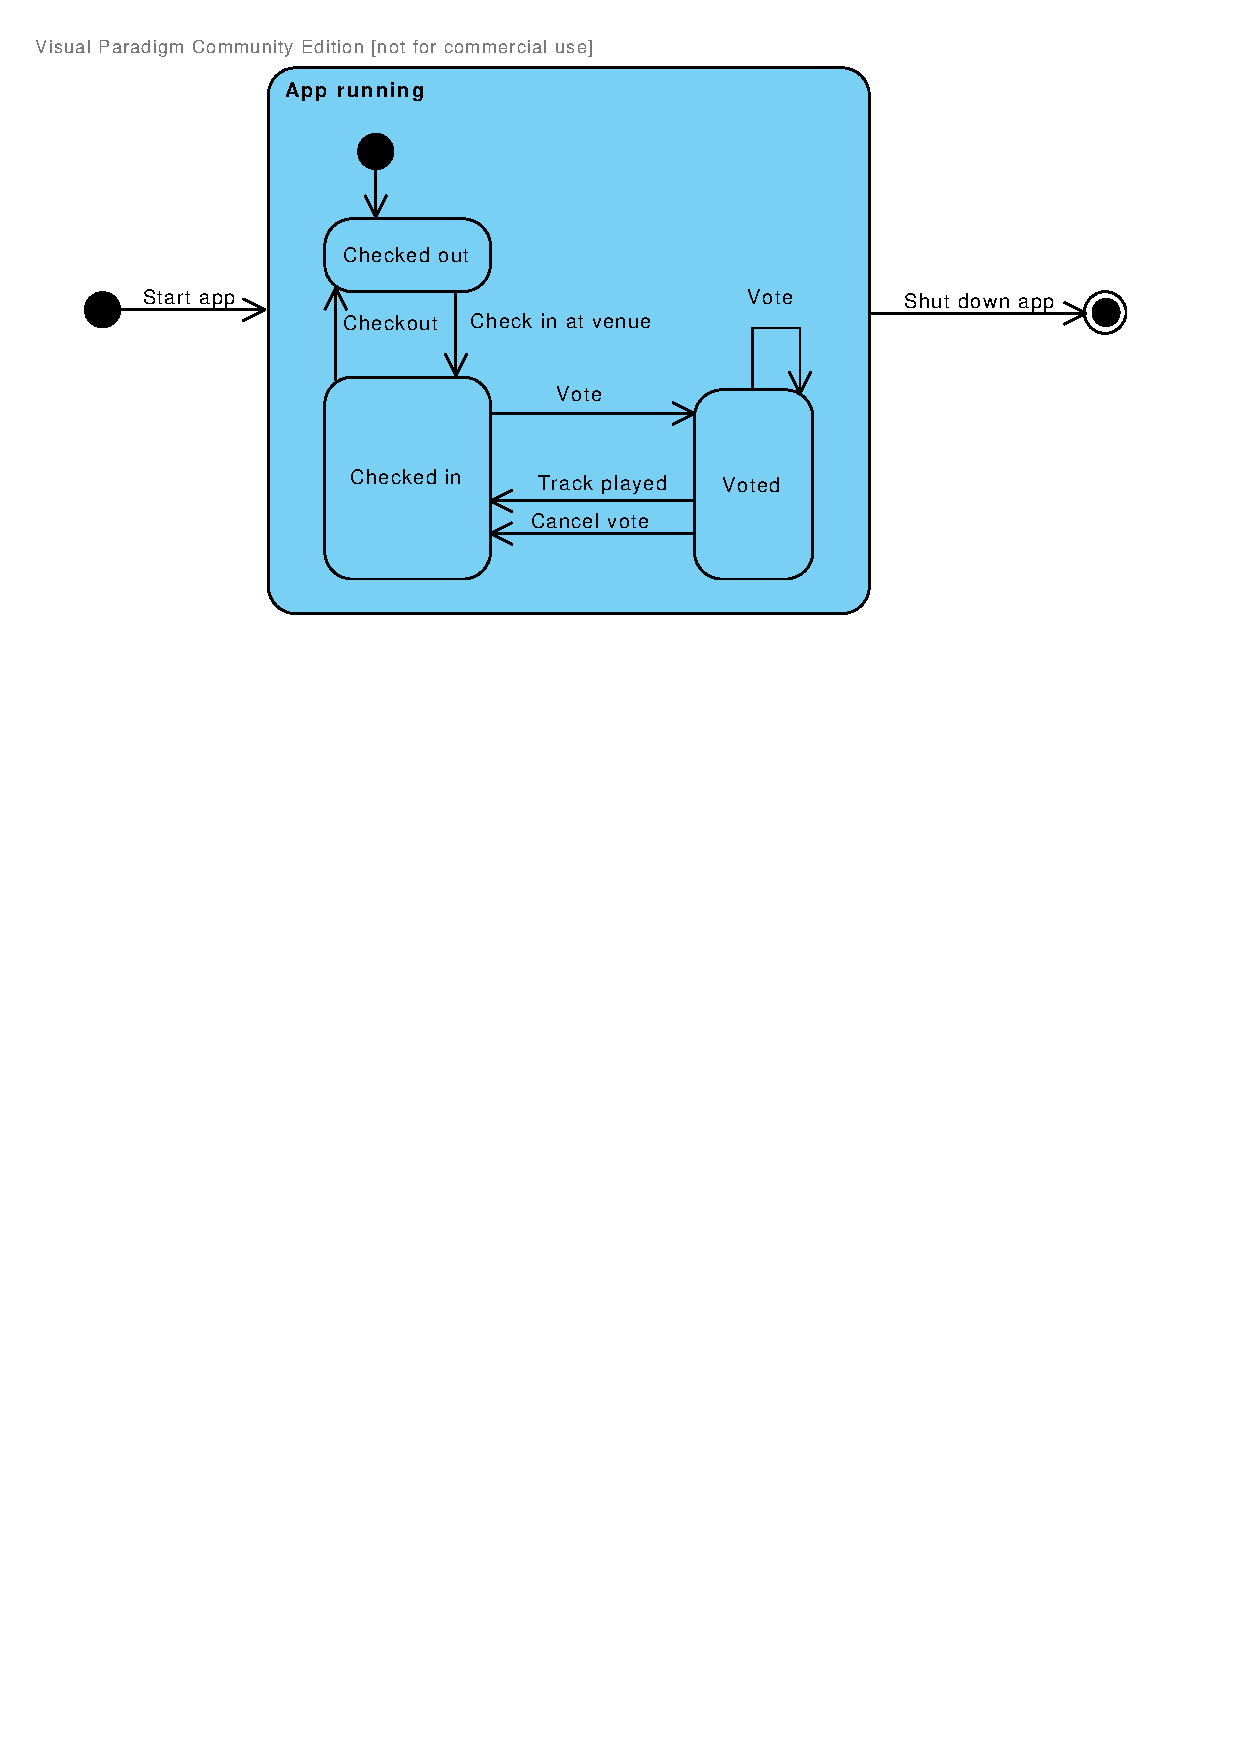
\includegraphics[width=1.1\linewidth]{Images/UsageUser.pdf}
  \caption{Usages for a guest.}\label{fig:UsageUser}
\end{figure}

\subsection{Use Case Specifications}

\actortable{Play Music}{
  The \emph{play music} use case is initiated by an administrator when music should start playing at the venue. This is done by pressing the play button on the administrator interface.
}

\actortable{Stop Music}{
  When an administrator wants to stop the music playing at the venue, the stop button on the administrator interface is pressed.
}

\actortable{Next Track}{
  If for some reason an administrator is not satisfied with the currently playing track, the next track button can be clicked to force a new track to be played.
}

\actortable{Add \& Remove Restriction}{
  Restrictions can be added to the system to disallow specific tracks to be played through the system. The administrator would do so whenever a certain theme of music has be complied to at the venue. These enforcements can later be removed.
}

\actortable{Check-in \& Check-out to Venue}{
  \emph{Check-in} to a venue is initiated by a guest to be able to interact with the music being played on a venue. The \emph{Check-in} is performed by pressing on a venue on a list on the guest application. \emph{Check-out} can either occur manually, by the user pressing a check-out button on the guest application, or the system can do it automatically.
}

\actortable{Vote \& Cancel Vote}{
  Guests at a venue can, when checked-in to the venue, vote on tracks to be played at the venue. This is done by finding a track that is already voted on, or searching for a track through the guest application.
}

\actortable{Influence Volume}{
  The volume of the music being played at a venue can be influenced both by an administrator, through the administrator interface, and by a guest, through the guest application. The guest may wish to lower the volume to be able to talk to fellow guests. An administrator may wish to override the volume wishes of guests, if for example the music is playing too low.
}
